% ECE 411
% Almatouq, Brooks, Forsman, Roman
% Fall 2019

% Document settings ------------------------------------------------
\documentclass[a4paper,12pt]{article}

% Commands ------------------------------------------------
\newcommand{\authorname}{Almatouq, Brooks, Forsman, Roman}
\newcommand{\classnumber}{ECE 411 - Group 18}
\newcommand{\projectname}{Project Theremizer}

\newcommand{\figOverlay}{\put(34,10){\color{black!50} \figWatermark}} % Figure overlay settings
\newcommand{\figWatermark}{\small \authorname \; \today} 		% Figure overlay text
\newcommand{\figHere}{\begin{overpic}[percent,scale=0.34]}	% Settings for all figures
\newcommand{\figHereB}{\begin{overpic}[percent,scale=0.5]}	% A different setting

% Packages ------------------------------------------------

\usepackage[USenglish]{babel} 	% American English
\usepackage{blindtext}			% Generate latin crap
\usepackage[yyyymmdd]{datetime} % Sets date format to ISO 8601 standard
\renewcommand{\dateseparator}{-}% Sets date format to ISO 8601 standard

\usepackage{graphicx}			% Image importing and display
\graphicspath{ {images/} }		% Path to image folder
\usepackage{xcolor}				% Allows normal color words
\usepackage{color, colortbl}

\usepackage{float}				% Adds 'H' for figure placement location
\usepackage{enumitem}			% Use for QandA environment
\usepackage{booktabs}			% Merging columns in tables
\usepackage{pdfpages}			% Add a PDF

\usepackage[firstpage]{draftwatermark}	% use [nostamp] when finished, [firstpage] otherwise
\SetWatermarkText{DRAFT}
\SetWatermarkColor{red!50}
\SetWatermarkScale{3}

\usepackage{overpic}				% Puts text over figures
\usepackage[american]{circuitikz}	% American-style circuit diagrams

\usepackage{amsmath}				% Multi-line equations
\usepackage{caption}				% Equation caption formatting
\usepackage{physics}				% Easier derivatives
\usepackage{gensymb}				% Enable \degree for degree symbol
\usepackage{siunitx}				% SI units


\usepackage{array}					% Used for centering tabular data
\newcolumntype{M}[1]{>{\centering\arraybackslash}p{#1}} % The actual centered column format

\usepackage{listings} %For code in appendix

\definecolor{mymauve}{rgb}{0.58,0,0.82}
\definecolor{mygreen}{rgb}{0,0.6,0}
\definecolor{mygray}{rgb}{0.5,0.5,0.5}
\definecolor{ltgray}{rgb}{0.937, 0.937, 0.956}	% Divide standard RGB values by 255 for some reason 

% PSU colors
\definecolor{PSUgreen}{RGB}{106,127,16}
\definecolor{PSUltgreen}{RGB}{168,180,0}
\definecolor{PSUblue}{RGB}{0,117,154}
\definecolor{PSUltblue}{RGB}{161,216,224}
\definecolor{PSUgray}{RGB}{71,67,52}
\definecolor{PSUbrown}{RGB}{96,53,29}
\definecolor{PSUsienna}{RGB}{163,63,31}
\definecolor{PSUred}{RGB}{210,73,42}
\definecolor{PSUorange}{RGB}{220,155,50}
\definecolor{PSUyellow}{RGB}{230,220,143}
\definecolor{PSUtan}{RGB}{232,221,162}
\definecolor{PSUpurple}{RGB}{101,3,96}


\newenvironment{QandA}
	{\begin{enumerate}[label=\arabic*.]\sl} % Use slanted question text and Arabic numerals
  {\end{enumerate}}
\newenvironment{answered}{\par\normalfont}{} % Paragraph break and use normal font

% fancy header / footer lines
\usepackage{fancyhdr}% http://ctan.org/pkg/fancyhdr
\pagestyle{fancy}% Change page style to fancy
\fancyhf{}% Clear header/footer
\fancyhead[L]{\textcolor{PSUgray}{\classnumber}}
\fancyhead[R]{\textcolor{PSUgray}{\projectname}}
\fancyfoot[L]{\textcolor{PSUgray}{\authorname}}
\fancyfoot[R]{\textcolor{PSUgray}{\thepage}}
\renewcommand{\headrulewidth}{0.4pt}% Default \headrulewidth is 0.4pt
\renewcommand{\footrulewidth}{0.4pt}% Default \footrulewidth is 0pt


% Title Page ------------------------------------------------
\begin{document}
\lstset { %Formatting for code in appendix
  language=Matlab,
  basicstyle=\footnotesize\ttfamily,
  numbers=left,
  stepnumber=1,
  showstringspaces=false,
  tabsize=1,
  breaklines=true,
  breakatwhitespace=false,
  stringstyle=\color{mymauve},
  keywordstyle=\color{blue},
  commentstyle=\color{mygreen}, 
}

\begin{titlepage}
	\begin{center}
		\vspace*{1cm}

		\huge\textsc{\projectname \\ Product Design Summary}

		\vspace{0.5cm}
		\small\textsc{\classnumber}
		
		\vspace{1.5cm}
		\normalsize \authorname 
		
		\vspace{0.5cm}
		%Lab TA: N/A
		
		\vfill
		\vspace{0.8cm}
		
		
\includegraphics[width=0.5\textwidth]{images/psulogo_horiz_msword.tif}
		
		\vspace{0.5cm}
		Electrical and Computer Engineering\\
		Portland State University\\
		\today
		 
	\end{center}
\end{titlepage}

% Table of contents ------------------------------------------------
\newpage
\tableofcontents


% Begin paper ------------------------------------------------
\newpage
\pagenumbering{arabic}

	\section{Executive Summary}
	Theremizer is a sound control and manipulation device. It's a small box, roughly the size of half a carton of eggs, with a 3-foot antenna protruding out the top, and various controls in front. It produces an audio output that sounds mysterious, ethereal, and otherworldly. Similar sounds have been used in famous and recognizable songs such as the theme from the Star Trek original series and the Beach Boys' "Good Vibrations". The user controls Theremizer by moving their hand in the physical space around its antenna, though never needing to touch the device directly. Theremizer interprets these motions and it uses it to change the pitch it produces. Theremizer also accepts an external audio input, and if provided, will modulate this external audio input using amplitude modulation to create wild sounds and effects. Theremizer's output is then run through a classic Voltage Controlled Filter, the AS 3220. This shapes the sound further using resonance and cutoff adjustments, for a distinctive, adjustable sound. Theremizer is primarily for modular synthesizer musicians, who are always looking for unique, interesting sounds and modular music boxes for live performances.
	\section{Market Analysis}
	\subsection{Target Market}
	Theremizer will be initially marketed to analog synthesizer enthusiasts, as they represent a large market of customers that are always looking for interesting audio sources and control methods. 

	\subsection{Sales}
	We aim to sell Theremizer for \$120.00, as devices with a smaller feature set are being sold for \$100 currently. We are adding features (filtering, modulation) that are highly desired in the modular synthesizer community, a community that has no problem spending significant money on devices. This device should be affordable to purchase in order to compete in an otherwise cost-prohibitive marketplace.
	\subsection{TAM / SAM / SOM}
	TAM: 8 million globally \\
	SAM: 180k musicians on the west coast \\ 
	SOM: 20k local musicians in the Portland area \\
	
	Note: Musicians, especially touring or performing musicians may be interested in multiple devices chained together or in various configurations.
	\subsection{Competition}
	There currently is nothing on the market that produces the same audio Theremizer can, at the competitive price point Theremizer has. Most theremins are disqualifyingly expensive and tonally limited. Cheaper devices don't have musical filtering on the output, or any modulation possibilities within the device. Both of these options limit the potential market for competitive devices. 
	
	\section{Requirements}
	\subsection{Functionality}
	An antenna must modulate the frequency of an oscillator which is heterodyned with another to produce an audio output of at least one octave. The device must be capable of feeding its output to other audio processing blocks, or a separate audio amplifier. The device must have an enclosure that is self-stable. The device should accept and modulate an external signal, then mix against the theremin output.
	\subsection{Performance}
		To make the device useful for musicians, it will have a user controlled filter with a minimum cutoff of at least \SI{5}{\kilo\hertz}. It will have a user controlled output up to at least \SI{1}{\volt} amplitude. The output and input impedance will be compatible with industry line-level standards and will have an impedance of less than \SI{600}{\ohm} and greater than \SI{10}{\kilo\ohm} respectively. 
	\subsection{Economic}
	The device must be affordable to produce, with a total parts cost less than \$60. All parts must be available for volume purchase, in active production, or easily substitutable by a component in current production. 
\section{System Architecture}
	\begin{figure}[H]
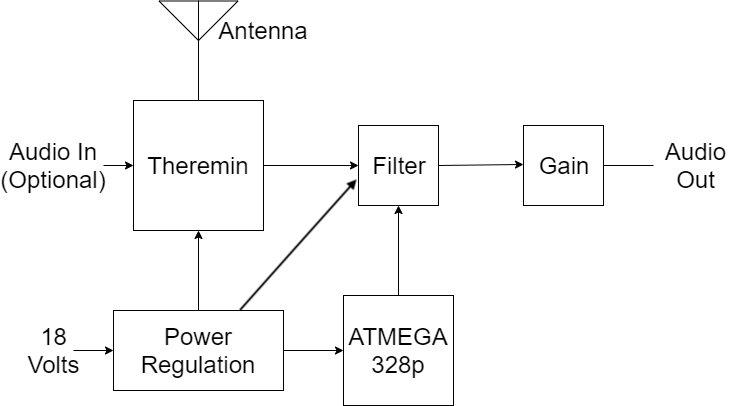
\includegraphics[width = \textwidth]{Theremizer_HighLevel_BD.png}
	\end{figure}

\section{Design Specification}
\begin{itemize}
	\item Sensors will be the antenna in the theremin circuit, and the ADC's on the processor. Antenna will input varying capacitance based on hand distance to theremin, and ADC's will measure voltage to vary PWM from the ATMega328p to control filter cutoff, resonance and gain.
	\item Actuators will be the mixer/modulator used in the theremin circuit (currently MC1496) which will output the modulated signal, the gain stage of the filter (AS3320), and the PWM output of the ATMega328p.
	\item Processors will be the ATMega328p and the filter, the AS3320.
	\item Power will be supplied by an \SI{18}{\volt} wall transformer and regulated by two switching regulators, one for the $\pm$ \SI{15}{\volt} required for the filter and theremin and one for the \SI{5}{\volt} required for the ATMega.
	\item We will attempt to program the ATMega without using the Arduino bootloader, but may switch if neccessary. 
	\item We will use Atmel/AVR Studio to write the code and program the processor.
\end{itemize}
\end{document}
